\documentclass{sig-alternate-05-2015}

\begin{document}

\title{CS265 Final Project}
\subtitle{Optimizing Memory Allocation Between Memtable, Cache, and Bloom Filters}
\numberofauthors{3}
\author{
\alignauthor
Mali Akmanalp\\
       \affaddr{Harvard University}\\
       \email{mea590@g.harvard.edu}
\alignauthor
A. Sophie Hilgard\\
       \affaddr{Harvard University}\\
       \email{ash798@g.harvard.edu}
\alignauthor Andrew Ross\\
       \affaddr{Harvard University}\\
       \email{andrew\_ross@g.harvard.edu}}

\date{\today}

\maketitle

\section{Introduction}
Tuning data systems is hard. Even for systems like key-value stores that only
support the most minimal API (\texttt{put} and \texttt{get}), the possibilities
are often overwhelming. The developers of RocksDB \cite{facebook:rocksdb}, a
popular and powerful key-value store, freely admit that ``configuring RocksDB
optimally is not trivial,'' and that ``even [they] as RocksDB developers don't
fully understand the effect of each configuration change''
\cite{rocksdb-tuning-guide}. Configurations must be optimized with respect to a
given \textit{workload}, which is rarely known in advance, although it is
sometimes roughly characterizable. There has been recent work \cite{monkey} in
determining the optimal memory allocation for bloom filters in terms of
worst-case analysis and with respect to a number of basic workloads, but
realistic key-value store workloads, which have been analyzed e.g. for Facebook
\cite{characterizing-memcached}, exhibit enormous complexity with respect to
time, skewness, and key repeatability.

Our goal is somewhat ambitious -- we seek to optimize not just bloom filter
memory allocation but memory allocation across the entire key-value store (to
cache, memtable, bloom filters, and possibly even fence pointers), and to do it
with respect to workloads we model as stochastic processes.

\section{Workloads}

Here are a number of basic workloads we will use to generate queries to
benchmark our key-value store in Python simulations. For
the simpler ones, we will also attempt to predict performance and derive
optimal parameters analytically.

\textbf{Uniform} queries will be drawn uniformly from keys $k \in
\{0,1,...,K\}$, where $K$ is a maximum key (that we explore varying). When we
draw a particular key $k_i$ for the first time, we will insert it into the
database as a write, and subsequently we will treat it as a lookup. Later we
will explore making a certain fraction of these queries into updates. The case
of uniformly distributed queries is often one in which the cache is unhelpful,
but in practice is highly unrealistic. Nevertheless, this is the scenario that
many analyses assume for calculations of big O complexity.

\textbf{Round-Robin} queries are drawn deterministically using $k_i = (i \mod
K)$, i.e. we iteratively draw each key in sequence, then repeat. This is also a
bad case for our key-value store in its default configuration; the fact that a
key has been recently written or read is actually a contraindication we will
access it again.

\textbf{80-20} queries (which are considered in \cite{monkey}) are drawn such
that 20\% of the most recently inserted keys constitute 80\% of the lookups.
This is a simple model we will be able to analyze analytically that exhibits
more realistic skew.

\textbf{Zipf} queries are distributed according to a Zipf or zeta distribution,
where the probability of a given key $k$ is $\propto \frac{1}{k^s}$, where $s
\in (1, \infty)$ describes the skewness of the distribution; in the limit
$s=1$, it is uniform with $K=\infty$. Zipf-distributed queries are considered
in \cite{art} as another simple proxy for realistically skewed queries.

\textbf{Discover-Decay} queries are distributed according to the following
stochastic process, inspired by the Chinese Restaurant process \cite{crp} but
with time decay: with every passing time increment $\Delta t \sim
\textrm{Expo}(\lambda_t)$, $n \sim \textrm{Pois}(\lambda_n)$ new keys are written to the
key-value store, which each have an inherent popularity $\theta_i \sim
\textrm{Beta}(a_\theta,b_\theta)$ with a random decay rate $\gamma_i \sim
\textrm{Beta}(a_\gamma,b_\gamma)$ that determines the exponential rate at which they
become less popular. The probability of drawing each $k_i$ is given by
$p(k_i,t) \propto \theta_i\gamma_i^{t-t_i}$, where $t$ is the current time and
$t_i$ is when the key was inserted. At each time step we sample $N$ keys from
$\textrm{Mult}(\{p(k_i,t)\})$. This stochastic process is somewhat arbitrary and we
hope to make it more realistic, but it does capture many of the essential
behaviors we know characterize key-value stores: new keys are constantly
inserted, some keys are much more popular than others, and the popularity of
most keys decays over time. The nonparametric nature of this stochastic process
may make inference difficult, and we also hope to enhance it to make it more
well-suited to realistic workloads (e.g. that exhibit daily periodicity), but
it seems much more able to simulate the richness of realistic queries than many
of the other models.

\section{Simulations}

We implemented a basic simulator of an LSM tree in Python \cite{lsmulator},
which simulates how an LSM tree with a variably sized cache, memtable, disk
layers, and bloom filters performs for an arbitrary sequence of queries. In
particular, we are able to simulate how often we are forced to access data on
disk (the main performance bottleneck for an LSM tree) and how often we can
respond with data in memory. So far, results suggest that the same LSM tree
architecture performs very differently under different query distributions
(Figure \ref{fig:sametree-diffqs}), and that different LSM tree architectures
perform very differently under the \textit{same} query distribution (Figure
\ref{fig:sameqs-difftree}). 
%We are working on an optimization procedure to find
%the best architecture for a given set of queries.

\begin{figure}[!htb]
\begin{center}
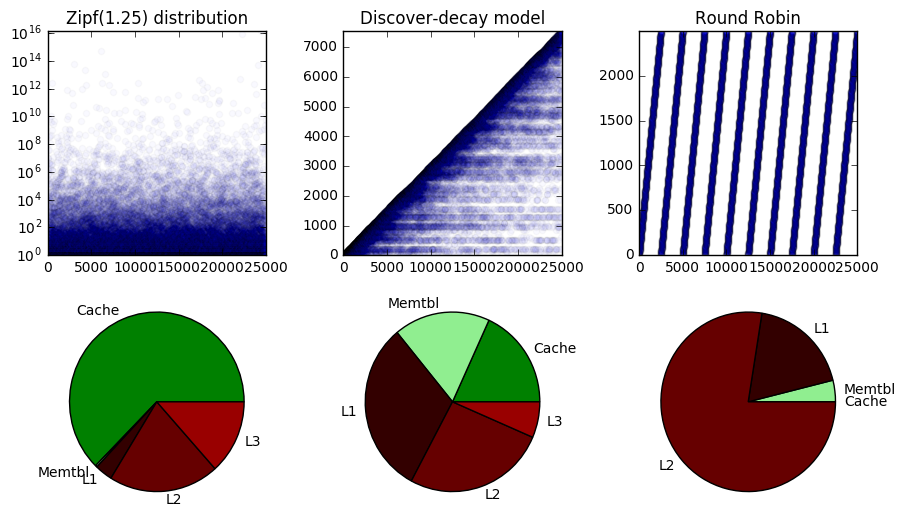
\includegraphics[width=9cm]{sametree-diffqs.png}
\end{center}
\caption{The same LSM tree architecture (a 25-element cache, 100-element
memtable, 5x layer ratio, and 10-bit bloom filters with 5 hash functions)
performs very differently for different query distributions. Memtable and cache
hits (in green) are fast, whereas accesses to the layers (in red) are slow. For
the Zipf workload, the cache is much more useful than the memtable, while the
situations are reversed for the Round-Robin workload. Both are useful in the
discover-decay case.}
\label{fig:sametree-diffqs}
\end{figure}

\begin{figure}[!htb]
\begin{center}
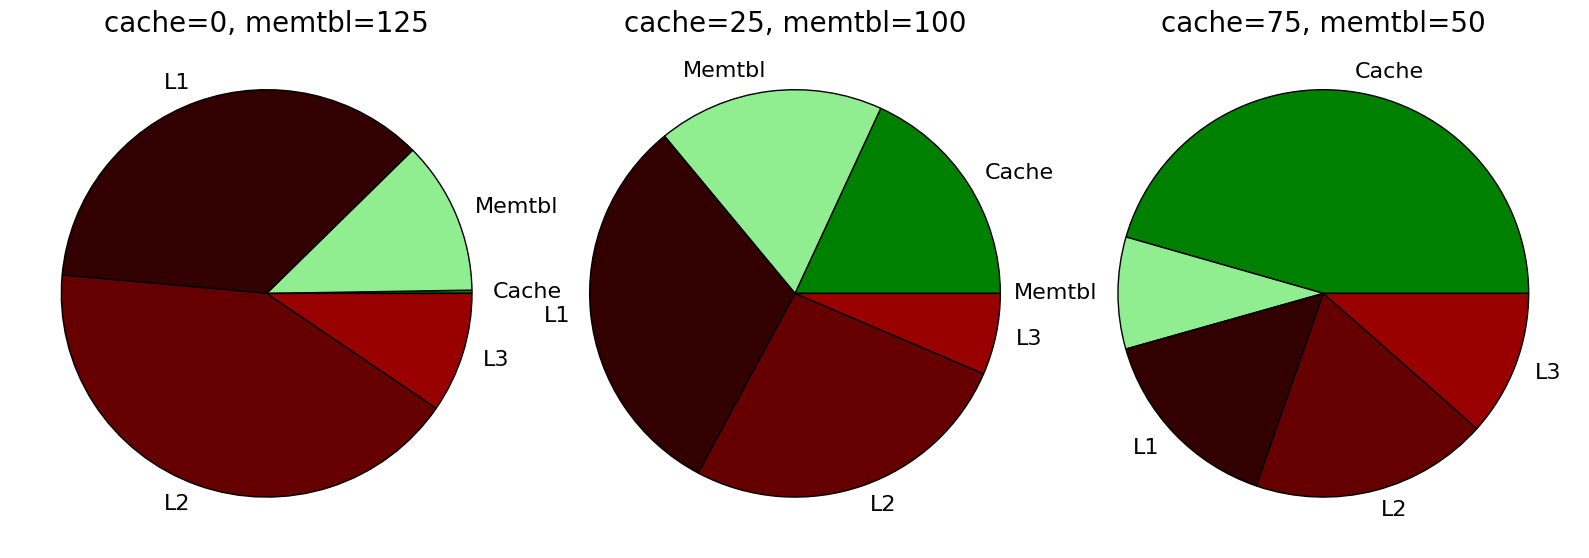
\includegraphics[width=9cm]{sameqs-difftree.png}
\end{center}
\caption{Performance results for different LSM tree architectures on the
discover-decay workload. Note that for this time-dependent workload, both the
cache and the memtable are useful, but finding the best ratio may require
optimization.}
\label{fig:sameqs-difftree}
\end{figure}

To find the distribution between memtable, bloom filters, and cache that minimizes memory accesses for a given workload, we create a simulation which iterates through the possible allocations of memory given a total memory size, using both Monkey and RocksDB default bloom filter layer allocations for a given bloom filter memory size. 

The resulting surfaces suggest that for some workloads, local optimization (that is, gradient descent) can be effective for moving toward an optimal memory allocation without requiring that we iterate through all possibilities. Additionally, we note that to compute iterative local optimizations, we do not require that the entire workload be known a priori. Rather, we can collect minimal statistics throughout the query execution process and use these to estimate the current value in saved I/Os any marginal byte of the cache, bloom filters, or memtable is providing. To formulate the useful statistics, we turn to modeling.

%\section{Benchmarking}
%
%So far, we've succeeded in getting basic benchmarks for RocksDB running and
%identifying which configuration parameters to vary. Our next step will be
%to generate queries in RocksDB format that correspond to our probabilistically
%modeled workloads, run them against RocksDB under different configurations
%that correspond to simulation parameters, and see if results match at least
%qualitatively.

\section{Modeling}

%Ideally, instead of resorting to simulation, we should be able to analytically compute the expected cost (in disk reads) of reading an element from our LSM tree. The following sections show some of our initial results under different assumptions about the query distribution. By the end of this project, we hope to show concordance between these results, simulations, and experiments with RocksDB.
We first consider the case of a uniform query distribution and then show how the formulation can be generalized to any distribution with an empirical trace.

\subsection{Uniform query distribution}

\noindent Assuming we have
\begin{itemize}
\item $N$ items in total DB \\
\item $E$ size of an entry in bits \\
\item $M$ total memory \\
\item $M_c$ memory allocated to cache \\
\item $M_{buffer}$ memory allocated to buffer\\
\item $P$ size of the buffer in pages \\
\item $B$ entries that fit in a disk page \\
\item $T$ ratio between layers of LSM tree such that \\
%  \item $n_t$ total items in the database
%  \item $n_c$ items that fit in cache
%  \item $n_m$ items that fit in memtable
%  \item a ratio $R$ between layers of LSM tree such that
  \item $L1 = T * B* P$, $L2 =T^2 * B*P $, and so on,
\end{itemize}

\noindent then we can solve for $L$ the total number of layers required to store all the data: \\
$$B*P * \frac{1-T^L}{1-T} = N$$
$$L= \lceil \textrm{log}_{T} \left(\frac{N(T-1)}{PB} + 1\right) \rceil$$


The average cost of a write remains the same as for the basic LSM tree case:
$$
\text{write cost} = \textrm{log}_{T} \frac{N}{BP}
$$

The average cost of a read must be considered probabilistically over all possible locations of the read item, in this case assuming a uniformly random distribution of reads:
\begin{itemize}
\item Probability that read is in memtable $= p(\text{MT}) = \frac{B*P}{N}$
\item Probability that read is in cache $= p(\text{cache}) = \frac{M_c/E}{N}$
\item Probability that read is in L1 but not in cache $= p(L1)$ $$= \frac{B*P * T - \frac{B*P*T}{N-B*P} * M_c/E}{N}$$
\end{itemize}
where the numerator is the number of items $B*P*T$ that are in the first layer minus the proportion of items from that layer that are probabilistically in the cache already: $$\frac{B*P*T}{N-B*P} * M_c/E$$
and finally where the $N-B*P$ comes from the fact that items already in memtable (L0) are not allowed to occupy the cache.

Therefore, given a uniform query distribution, the full expected cost in disk reads of a read is
$$E[C_{\text{uniform}}] = p(\text{MT}) * 0  + p(\text{cache}) * 0 + \sum_{i=1}^L p(L_i) * i$$
$$=\sum_{i=1}^L \frac{B*P * T^i - \frac{B*P*T^i}{N-B*P} * M_c/E}{N} * i$$

%\subsection{Uniform query distribution}
%
%\noindent Assuming we have
%\begin{itemize}
%\item $N$ items in total DB \\
%\item $E$ size of an entry in bits \\
%\item $M$ total memory \\
%\item $M_c$ memory allocated to cache \\
%\item $M_{buffer}$ memory allocated to buffer\\
%\item $P$ size of the buffer in pages \\
%\item $B$ entries that fit in a disk page \\
%\item $T$ ratio between layers of LSM tree such that \\
%%  \item $n_t$ total items in the database
%%  \item $n_c$ items that fit in cache
%%  \item $n_m$ items that fit in memtable
%%  \item a ratio $R$ between layers of LSM tree such that
%  \item $L1 = T * B* P$, $L2 =T^2 * B*P $, and so on,
%\end{itemize}
%
%\noindent then we can solve for $L$ the total number of layers required to store all the data: \\
%$$B*P * \frac{1-T^L}{1-T} = N$$
%$$L= \lceil \textrm{log}_{T} \left(\frac{N(T-1)}{PB} + 1\right) \rceil$$
%
%
%The average cost of a write remains the same as for the basic LSM tree case:
%$$
%\text{write cost} = \textrm{log}_{T} \frac{N}{BP}
%$$
%
%The average cost of a read must be considered probabilistically over all possible locations of the read item, in this case assuming a uniformly random distribution of reads:
%\begin{itemize}
%\item Probability that read is in memtable $= p(\text{MT}) = \frac{B*P}{N}$
%\item Probability that read is in cache $= p(\text{cache}) = \frac{M_c/E}{N}$
%\item Probability that read is in L1 but not in cache $= p(L1)$ $$= frac{B*P * T - \frac{B*P*T}{N-B*P} * M_c/E}{N}$$
%\end{itemize}
%where the numerator is the number of items $B*P*T$ that are in the first layer minus the proportion of items from that layer that are probabilistically in the cache already: $$\frac{B*P*T}{N-B*P} * M_c/E$$
%and finally where the $N-B*P$ comes from the fact that items already in memtable (L0) are not allowed to occupy the cache.
%
%Therefore, given a uniform query distribution, the full expected cost in disk reads of a read is
%$$E[C_{\text{uniform}}] = p(\text{MT}) * 0  + p(\text{cache}) * 0 + \sum_{i=1}^L p(L_i) * i$$
%$$=\sum_{i=1}^L \frac{B*P * T^i - \frac{B*P*T^i}{N-B*P} * M_c/E}{N} * i$$
%$$= \sum_{i=1}^L \frac{n_m * R^i - \frac{n_m * R^i}{n_m * \frac{1-(R^j-1)}{1-R}} * n_c}{n_t}  * i$$

%\subsection{Skewed Reads (80-20)}
%
%Now consider the case for skewed reads, where we say $d_{hf}$ ($d_{lf}$) percent of the data ($hf \equiv$ high-frequency) receives $r_{hf}$ ($r_{lf}$) percent of the reads (where $d_{hf} + d_{lf} = 1$ and $r_{hf} + r_{lf} = 1$). On average, we can assume that the cache contains $r_{hf} * n_c$ items from $d_{hf} * n_t$ and $r_{lf} * n_c$ items from $d_{lf} * n$. Then the expected cost of a read is dependent on whether the data item being read is in $d_{hf} * n_t$ or $d_{lf} * n$ as the probability of a cache hit varies.\\ \\
%Concretely, consider where we have 3 levels and 800 total items with a cache of size 10 and a ratio of 2  (for L0=100, L1 = 200, L2 = 400 items), with $d_{hf} = .2$ and $d_{lf} = .8$ and $r_{hf}$ = .8 and $r_{lf}$ = .2, which matches the scenario considered in \cite{monkey}. Then the cache, on average, contains 8 items from $d_{hf} * n$ and 2 items from $d_{lf}*n$. If we execute a read on one of the 200 items in $d_{hf}$, then, there is a $\frac{8}{200}$ chance that that item is in the cache. If we execute a read on one of the $200*\frac{1}{4} = 50$ items of  $d_{hf} * n_t$ in L1, we expect that $\frac{2}{6} * 8$ of those items would have actually been found already in cache, as this level contains $\frac{2}{6}$ of all of the items not in the memtable. Then the probability that a read is found in L1 is the proportion of the $d_{hf} * n_t = 160$ items that will reside in L1 but not in the cache, which is $\frac{40 - \frac{2}{6} * 8}{160}$. \\ \\
%Just limiting ourselves to high-frequency data, we see that:
%\begin{itemize}
%  \item Probability that read is in memtable $= p(\text{MT}_{hf}) = \frac{B*P*d_{hf}}{d_{hf} *N}$
%  \item Probability that read is in cache $= p(\text{cache}_{hf}) = \frac{r_{hf} * M_c/E}{d_{hf} * N}$
%  \item Probability that read is in $L_i$ but not in cache $= p(L_{i,hf})$ $$ = \frac{B*P * T*d_{hf} - \frac{B*P * T}{N-B*P} * r_{hf} * M_c/E}{d_{hf} * N} $$
%\end{itemize}
%
%This gives us the final expected cost of reading high frequency items:
%$$
%\begin{aligned}
%E[C_{\text{skew}, hf}]
%& = p(\text{MT}_{hf}) * 0  + p(\text{cache}_{hf}) * 0 + \sum_{i=1}^L p(Li_{hf}) i \\
%& = \sum_{i=1}^L \frac{B*P * T^i*d_{hf} - \frac{B*P * T^i}{N-B*P} * r_{hf} * M_c/E}{d_{hf} * N} * i
%%& = \sum_{i=1}^j \frac{n_m * R^{i}*d_{hf} - \frac{n_m * R^{i}}{n_m * \frac{1-(R^j-1)}{1-R}} r_{hf} n_c}{d_{hf} n_t} i
%\end{aligned}
%$$
%
%The expected cost of reads for low-frequency items can be enumerated analogously, and combining the expectation of reads in $d_{hf}$ and $d_{lf}$, we obtain
%$$
%E[C_{\text{skew}}] = r_{hf} * E[C_{\text{skew}, hf}] + r_{lf} * E[C_{\text{skew}, lf}],
%$$
%
%which is the expected number of lower layer accesses per read on a workload where $d_{hf}$ percent of the data receives $r_{hf}$ of the reads.

\subsection{Bloom Filters}

The previous analysis hasn't yet accounted for the presence of Bloom filters, which reduce the likelihood we will unnecessarily access a lower layer. For a Bloom filter of $k$ bits with $h$ independent hash functions $h_1, h_2,...h_h$, the probability that a given bit is still set to 0 after inserting $n$ keys is 
$$
(1 - \frac{1}{k})^{n*h}
$$
Then the probability of a false positive is 
$$
(1- (1 - \frac{1}{k})^{n*h})^h \approx (1 - e^{-hn/k})^h
$$

We can minimize this over $h$ to find the optimal number of hash functions, which is $h = \mathrm{ln}(2) * \frac{k}{n}$. Assuming that this is the number of hash functions $h$ we will use, the probability of a false positive as a function of the number of bits is then 
$$
(1 - e^{-\mathrm{ln}(2)*k/n*n/k})^{\mathrm{ln}(2) * \frac{k}{n}} = (\frac{1}{2}) ^ {\mathrm{ln}(2) * \frac{k}{n}} \approx (.6185) ^  {\frac{k}{n}}
$$

For an item in any any level $L_i$ of the LSM tree with $i \geq 2$ we can reduce the expected cost of accessing that item from $i$ by the number of Bloom filter negatives at any level $j<i$. \\ \\
Then the expected cost of accessing an item at $L_i$ is  $$\sum_{j=1}^{i-1} p(fp_j) * 1 + 1$$
Where $p(fp_j)$ is the probability of a false positive for that key at level $j$ and 1 is the cost of actually accessing the item at level $i$ assuming fence pointers that lead us to the correct page.

\subsection{Expected Cost with Bloom Filters - Base Case}

Assuming a random distribution of reads, we now consider also the probability that a bloom filter allows us to ignore a level: \\
%\begin{itemize}
%  \item Probability that read is in memtable $= p(\text{MT}) = \frac{B*P}{N} $
%  \item Probability that read is in cache $= p(\text{cache}) = \frac{M_c/E}{N}$
%  \item Probability that read is in $L_i$ but not in cache $= p(L_{i})$ $$ = \frac{B*P*T^i - \frac{B*P*T^i}{N-B*P} * M_c/E}{N}  $$
%\end{itemize}
Expected cost of read for an item in the tree = $$p(mt) * 0  + p(cache) + 0 + \sum_{i=1}^L p(Li) * \sum_{j=1}^{i-1} p(fp_j)$$ \\
Expected cost for a null result read = $\sum_{j=1}^{L} p(fp_j)$

Given a total memory allocation $M$, the total number of bits we can allocate to bloom filters is $M-M_c = \sum_{i=1}^L m_i$ \\
Then the total formula for the expected cost of a read in the tree is: 
\begin{multline}
$$E[c] = \sum_{i=1}^{L} \frac{B*P*T^i - \frac{B*P*T^i}{N-B*P} * M_c/E}{N} \\ \cdot \left[ \left(\sum_{j=1}^{i-1} (.6185) ^  {\frac{m_j}{B*P*T^j}}\right) +1 \right]$$ 
\end{multline}
Whereas with a given percentage of null reads in the workload $p_{null}$:
\begin{multline}
$$E[c] = (1-p_{null})\sum_{i=1}^{L} \frac{B*P*T^i - \frac{B*P*T^i}{N-B*P} * M_c/E}{N} \\ \cdot \left[ \left(\sum_{j=1}^{i-1} (.6185) ^  {\frac{m_j}{B*P*T^j}}\right) +1 \right] + p_{null}\sum_{j=1}^{L} p(fp_j)$$
\end{multline}
\begin{multline}
$$E[c] = \sum_{i=1}^{L} (1-p_{null})\frac{B*P*T^i - \frac{B*P*T^i}{N-B*P} * M_c/E}{N} \\ \cdot \left[ \left(\sum_{j=1}^{i-1} (.6185) ^  {\frac{m_j}{B*P*T^j}}\right) +1 \right] + p_{null} \cdot p(fp_i) $$
\end{multline}
%We'd like to minimize this subject to the constraint that $M_c + \sum_{i=1}^L m_i = M$ \\
%(This assumes all levels are full at all times: should we assume half full on average?)

%\subsection{Expected Cost with Bloom Filters - Skewed Reads}
%
%Expected cost of read on item in $d_{hf}$: 
%\begin{multline}
%$$E[C_{hf}]=  \sum_{i=1}^L \frac{B*P * T*d_{hf} - \frac{B*P * T}{N-B*P} * r_{hf} * M_c/E}{d_{hf} * N} \\ \cdot \left[ \left(\sum_{j=1}^{i-1} (.6185) ^  {\frac{m_j}{B*P*T^j}}\right) +1 \right]$$
%\end{multline}
%The expected cost of a read on an item in $d_{lf}$ can be enumerated analogously, and we combine the expectation of reads in $d_{hf}$ and $d_{lf}$ as: \\
%Expected cost of read = 
%\begin{multline}
%$$ \sum_{i=1}^L r_{hf} *\frac{B*P * T*d_{hf} - \frac{B*P * T}{N-B*P} * r_{hf} * M_c/E}{d_{hf} * N} + \\ r_{lf} * \frac{B*P * T*d_{lf} - \frac{B*P * T}{N-B*P} * r_{lf} * M_c/E}{d_{lf} * N} \\ \cdot \left[ \left(\sum_{j=1}^{i-1} (.6185) ^  {\frac{m_j}{B*P*T^j}}\right) +1 \right]$$\end{multline}

\subsection{Expected Cost with Bloom Filters - Generalized Distribution}
Note that in the above, the workload specific factors are the probability that a read is at any given level and the related probability that any given item from a level is already in the cache. To compute an empirical estimation of the probability that any given item is in a layer but not already in the cache, we can simply keep statistics on the total number of times a key was found in that layer divided by the total number of (non-null) read queries executed. Then we can consider the following simplification:
\begin{multline}
$$E[c] = \sum_{i=1}^{L} (1-p_{null})\left[p(L_i) - \frac{p(L_i)}{(N - BP)} * M_c/E \right]\\ \cdot \left[ \left(\sum_{j=1}^{i-1} (.6185) ^  {\frac{m_j}{B*P*T^j}}\right) +1 \right] + p_{null} \cdot p(fp_i) $$
\end{multline}

Taking the derivative with respect to the number of entries in the cache, $M_c/E$, we get 
$$
- p(L_i)/(N - BP) \cdot \left[ \left(\sum_{j=1}^{i-1} (.6185) ^  {\frac{m_j}{B*P*T^j}}\right) +1 \right]
$$
Which is just the average cost of a read throughout the tree. Then, to keep statistics on how valuable we expect the cache to be, we maintain statistics on the average cost of every read performed in the window of interest.

Because the memory allocation problem is discrete anyway, we consider the value of the bloom filters as a finite difference, that is the approximate value of any marginal bloom filter bit at layer $k$ will be $E[c | m_k+1] - E[c | m_k]$. In this computation, all terms in the sums drop out except for those concerning $m_j$, and we are left with:
\begin{multline}
$$\sum_{i=k}^{L} (1-p_{null})\left[p(L_i) - \frac{p(L_i)}{(N - BP)} * M_c/E \right] \\ \cdot \left\{ \left[ \left( (.6185) ^  {\frac{m_k+1}{B*P*T^j}}\right) +1 \right] - \left[ \left( (.6185) ^  {\frac{m_k}{B*P*T^j}}\right) +1 \right] \right\} \\+ p_{null}  \left( (.6185) ^  {\frac{m_k+1}{B*P*T^j}} - (.6185) ^  {\frac{m_k}{B*P*T^j}}\right)$$
\end{multline}

Rearranging terms, we get:
\begin{multline}
$$\sum_{i=k}^{L} \left[(1-p_{null})\left[p(L_i) - \frac{p(L_i)}{(N - BP)} * M_c/E \right] +  p_{null} \right] \\ \cdot \left( (.6185) ^  {\frac{m_k+1}{B*P*T^j}} - (.6185) ^  {\frac{m_k}{B*P*T^j}}\right)$$
\end{multline}

Where this is exactly the number of times the given bloom filter is accessed times the difference in the theoretical false positive rates given memory allocations $m_j$ and $m_j+1$. Then, to keep statistics on how valuable we expect any given bloom filter to be, we maintain statistics on the number of times every bloom filter was accessed in the window of interest.

To estimate the additional value of any marginal memory in the buffer with respect to reads, we must make a number of simplifications, as $P$, the number of pages in the buffer, factors into every term in this equation. Further, the interaction between $P$ and most of the terms is not available in closed form, in general. Rather, the critical terms $P(L_i)$ we are empirically estimating. Then, for reasonably large values of $N$ and $P$, we will assume that the bloom filter false positive rate stays approximately the same, as does the value of the cache. Then, we consider only the change in I/Os occurring from the altered probability of any given element occurring in any layer as a result of more elements being in the memtable. Further, we can provide a simple underestimate of this by assuming that any items we add to the memtable will be removed from otherwise occurring in L1, without considering the added value resulting cascade through all other values in all other layers of the table.

Then, an appropriate estimate of how useful any additional space of memory in the memtable is is simply the resulting change in $p(L_i)$ * 1 (as any element at L1 is accessed with a single I/O and no consideration of bloom filter false positive rates). To estimate how many additional times L1 would be accessed if we instead allocated the final portion of the memtable to L1, we keep statistics on how often the final spots of the memtable were accessed in a read. In practice, these spots are accessed only very infrequently, as the buffer is accessed only a handful of times at this stage before being flushed. This statistic might be more helpful on a system with constant compaction rather than a full layer flush.

For the buffer, we must additionally consider the saved update/insert I/Os. 
$$
 \text{write cost} = \textrm{log}_{T} \frac{N}{BP}
$$
Taking the derivative with respect to $BP$, the number of items in the buffer, we get $\frac{1}{BP}$
In discrete terms, this evaluates to $\textrm{log}_{T} \frac{BP}{BP+1}$. 

We consider additionally the fact that I/O savings are lessened by the number of duplicates inserted, as duplicates will not be merged the full length of the tree. To take this into account we also keep a statistic for the total number of duplicates merged over the window of interest and compute the expected number of saved I/Os for an increase in buffer as $\textrm{log}_{T} \frac{BP}{BP+1}$ * (number of puts - number of duplicates).
The only statistics we need to compute this are the empirical number of update queries and the empirical number of duplicates found and removed over the window of interest.
%\subsection{Variable Cache, Constant Layers}
%
%Now we want to analyze what happens when we vary the proportion of memory allocated to the cache and the memtable. Given a fixed memory size $n_v$, we first consider the simplification of assuming a constant layer structure. Of course, in general a larger memtable will allow for larger layers, affecting both read and write performance. Let $n_l$ be the size of the first layer when $n_v = n_m$ (all memtable) and $n_c =n_v - n_m$.\\ \\
%\textbf{Uniform Case:} \\
%%if we assume some fixed base layer size $n_l$, which is the size of the memtable if it exists.
%Consider the formula used earlier:
%$$
%p(\text{MT}) * 0  + p(\text{cache}) * 0 + \sum_{i=1}^j p(L_i) * i 
%$$
%
%In the extreme case where $n_m=0$ (\textbf{no memtable}), the formula in the numerator of the sum simplifies to be over $n$ the total number of items, as there is no memtable layer and the probability of the first layer now has a cost of 1. However, we now have to add a number of items to each level of the tree that sum to the amount that were in L0. We add them as a geometric series per layer to maintain the structure
%$$
%\sum_{i=i}^{j} \frac{(n_l) * R^{i} + \frac{(n_l) * R^{i}}{n_t} * n_v - \frac{(n_l) * R^{i}}{n_t} * n_v}{n_t} * (i)
%$$
%The two latter terms cancel and we are left with
%$$
%\sum_{i=1}^j \frac{(n_l) * R^i}{n_t} * i 
%$$
%In the extreme case of \textbf{no cache}, 
%$$
%\sum_{i=1}^j \frac{(n_l) * R^i}{n_t} * i 
%$$
%And we can see that this is in fact the same result as the no memtable case. \\ \\
%In general, for any selection of $n_m$ and $n_c$ we have
%\begin{multline}
%\sum_{i=1}^j \frac{(n_l) * R^i - \frac{(n_l) * R^i}{(n_l) * \frac{1-(R^j-1)}{1-R}} * (n_v-n_m)}{n_t} \\+
%\frac{\frac{(n_l) * R^i}{(n_l) * \frac{1-(R^j-1)}{1-R}} * (n_v-n_m)}{n_t} * i 
%\end{multline}
%and so with a random workload, the choice is irrelevant \textit{assuming a constant number of layers}. In actuality, with a larger memtable we will be able to decrease the total number of layers needed. \\
%\\
%\textbf{Skewed Reads (80-20) Case:}\\
%Now consider the case for skewed reads, where we say $d_{hf}$ ($d_{lf}$) percent of the data receives $r_{hf}$ ($r_{lf}$) percent of the reads (where $d_{hf} + d_{lf} = 1$ and $r_{hf} + r_{lf} = 1$). On average, we can assume that the cache contains $r_{hf} * n_c$ items from $d_{hf} * n_t$ and $r_{lf} * n_c$ items from $d_{lf} * n$. \\ \\
%In the extreme case of \textbf{no cache}, the result will be as above. \\ \\
%In the extreme case of \textbf{no memtable}, the expected cost of a read is dependent on whether the data item being read is in $d_{hf} * n_t$ or $d_{lf} * n$ as the probability of a cache hit varies.\\
%For data in $d_{hf} * n$, \\ \\
%Probability that read is in cache:
%$$\frac{r_{hf} * n_c}{d_{hf} * n_t} = p(\text{cache}_{hf})$$ \\
%Probability that read is in $L_i$ but not in cache: 
%\begin{multline}
%\frac{n_l * R^{i}*d_{hf} - \frac{n_l * R^{i}}{n_t} * r_{hf} * (n_v)}{d_{hf} * n_t} \\+ \frac{\frac{n_l * R^{i}}{n_t} *d_{hf} *(n_v)}{d_{hf} * n_t}  \\= \frac{n_l * R^{i}*d_{hf}+ \frac{n_l * R^{i}}{n_t} * (d_{hf}-r_{hf})* n_v}{d_{hf} * n_t} = p(Li_{hf}) 
%\end{multline} \\
%Expected cost of read on item in $d_{hf}$: \\
%$$E[C_{hf}]= p(\text{cache}_{hf}) * 0 + \sum_{i=1}^j p(Li_{hf}) * i$$\\
%$$
%= \sum_{i=1}^j \frac{n_l * R^{i}*d_{hf}+ \frac{n_l * R^{i}}{n_t} * (d_{hf}-r_{hf})* n_v}{d_{hf} * n_t}  * i
%$$ \\
%From this equation we can see that the probability (and thus the expected cost) is increasing in $d_{hf}$ and decreasing in $r_{hf}$. This makes sense, as for many reads (high $r_{hf}$) on a small amount of data (low $d_{hf}$) we would expect frequent cache hits. \\ \\
%For general memtable/cache allocation, probability that read is in $L_i$ but not in cache: 
%\begin{multline}
%\frac{n_l * R^{i}*d_{hf} - \frac{n_v * R^{i}}{n_l * \frac{1-(R^j-1)}{1-R}} * r_{hf} * (n_v - n_m)}{d_{hf} * n_t} \\+ \frac{\frac{n_v * R^{i}}{n_l * \frac{1-(R^j-1)}{1-R}} *d_{hf} *(n_v - n_m)}{d_{hf} * n_t}  = p(Li_{hf})
%\end{multline}
\section{Statistical Gradient Descent}
\subsection{Testing Accuracy and Variance of Statistics}
First we generate a variety of workloads against which to test the accuracy of our statistics in predicting the change in I/Os for increasing the memory allocated to a given data structure. In this context, we hold all other data structures constant and increase the total memory by one entry (64 bits), which we give to the data structure being analyzed. 

Results show wide dispersion around the predicted number of I/Os, which generally falls at or around the mean of the distribution.


\subsection{Testing Theoretical I/O Savings Against Simulation}
To test whether basic statistics are capable of accurately predicting proper memory reallocation based on workload, we add statistic collection for the statistics mentioned above to the simulator. Then, for points on the precomputed surface, we see what the expected I/Os would have been and what memory the heuristics above would have directed us to reallocate.

\section{Results}

\section{Future Work}
There are many additional optimizations we chose not to address for the moment in this problem. For example, what is the optimal time to reallocate memory? In an environment where we assume full flushing of a given layer and the recomputation of all bloom filters for the layers involved in the flush, it seems like this would be an optimal point to reallocate memory locally among the data structures that are being rewritten anyway. However, this leads to only rare opportunities to recompute deeper layers of the LSM tree, and in practice LSM tree layers are not actually flushed in this `all-at-once' fashion. 

Additionally, the equivalent to a stochastic gradient descent learning rate for our problem is the chunk size of memory that we allow to be reallocated at any calculation point. For now, we consider only the reallocation of the smallest available piece of memory. However, in situations where we have a large amount of conviction in the predictions and they show large potential gains, it might make more sense to reallocate a large block of memory at once. In this case, the reallocation strategy requires more thought than merely taking a chunk from the lowest value data structure and giving it to the highest value data structure. Optimally computing what that reallocation strategy would be would likely require a deeper set of statistics, showing a trend of value over the last portion of any of the data structures, rather than only the last key as we have been using.

Building on the above, there are a number of opportunities for storing histograms rather than simple rolling averages of statistics (in particular, we store a histogram of bloom filter accesses at each stage of bloom filter `fullness' to allow us to calculate the average false positive rate for any number of bits after the fact rather than rolling averages of expected false positive rates for a few potential memory allocations). Histograms are a much heavier statistic than a simple number but provide a greater flexibility in the reallocation stage. More work needs to be done to calculate how much added benefit could be achieved in practice from these costlier statistics and to find scenarios in which they might be worthwhile.

%What we have done so far is to analytically compute basic quantities (like the
%expected cost of individual reads) as a function of LSM tree attributes for
%basic query distributions. Once we extend this analysis to allow the number of
%layers to vary with the memtable size, we should be able to directly compare
%these analytic results to simulation and experimental benchmarks, and then
%finally attempt to derive optimal LSM tree parameters.

\section{Bringing it all together}

%Once we have analytic and simulated predictions of optimal RocksDB
%configurations that match benchmarking experiments, the final step will be to
%consider whether we can implement adaptive updating in RocksDB to optimize
%performance on the fly. We are considering several options, including on-the-fly
%inference and maintaining a small number of fixed parameter settings that we can
%dynamically decide between to simplify the problem.
%
%Overall, however, we believe even being able to determine the optimal LSM tree
%architecture in theory (based on a deep and accurate characterization of the
%workload) will be a useful contribution.

\bibliographystyle{abbrv}
\small
\bibliography{bibliography}

\end{document}
